\documentclass[a4paper]{article}
\usepackage[T1]{fontenc}
\usepackage[utf8]{inputenc}
\usepackage[top=2cm, bottom=2cm, left=2cm, right=2cm]{geometry}
\usepackage{color}
\usepackage{url}
\usepackage{array}
\usepackage{pifont}
\usepackage{graphicx}
\setlength{\skip\footins}{2cm}

\title{COMP-512 Distributed Systems, Fall 2011}
\author{
Matthieu \textsc{Dubet} \\
Alexander \textsc{Kawrykow} \\ \\ \\
\emph{School of Computer Science, McGill University }
}

\begin{document}
\maketitle
\begin{figure}
  \centering
	
\includegraphics[scale=0.8]{mcgill_logo.png}
  \caption{McGill University}
  \label{mcgill}
\end{figure}
\tableofcontents
\clearpage

%\section{Introduction}
\section{Project Part 1: Distributing an Application}
\subsection{Design}

We decided to separate the ResourceManager interface to split the concerns. 

Accordingly, we created one type of Interface for each kind of resource (room, car, flight, customer), and finally aggregated all these into one large interface (the IResourceManager). 

We then looked at the functionality common to anything Resource-Manager related: reading data, writing data, querying data, etc. In particular,
these are functions which have no semantic meaning specific to any of the resources. We extracted these into an AbstractResourceManager.
For each kind of resource, we implemented a concrete ResourceManager who was able to reuse the functionality in the AbstractResourceManager, 
but in the context of a particular resource. 


Both our RMI and TCP implementations of the ResourceManagers act as wrappers for their underlying ResourceManager. That is, a RMI car resource manager
takes care of binding to the registry and remote method calls, but the underlying logic happens by delegating to a concrete car resource manager. A
similiar approach was taken for the TCP car resource manager. In this way, we were able to maximize code reuse. 


Another step taken to maximize code reuse was our treatment of the Client. Rather than re-writing the client for TCP, we created a TCP "proxy" resource
manager which implements IResourceManager, but simply passes on the exact command to the remote middleware server. Here, the proxy is simply a local
reference we can create when the client is launched.


The remote middleware server listens for the TCP/IP messages, looks at the first few letters, and then delegates the exact command. For example, we know a command containing the substring "car" must be sent, via TCP/IP, to the car resource manager server, so little processing of the commands ever needs to take place. 

The car resource manager can then just look at the first few letters of his received command,
and delegate to his reference to a local concret car resourcemanager depending on the type of query. For example, if the command starts with 'new', we know
we can call the newCar method on the local reference and have him take care of the logic. 



To handle customers, we decided to treat the MiddleWare as a kind of resource manager himself. 

In both implementations, the Middleware server has a local reference to a CustomerResourceManager object to handle all of the logic pertaining to customers, as well as reservations and the itinerary feature. In the case of RMI, the CustomerResourceManager can use his remote object references to easily handle reservations. By contrast, for the TCP implementation, we had to reconstruct the objects the CustomerResourceManager would put in his hashtable. 

We did this by exchanging the objects over sockets in string form, as a list of attributes corresponding to the id, location, price, etc. For example, to reserve a car, the flow goes something like: send message to middleware, middleware constructs Car object by sending message to car resource manager to obtain the state of the specific car, middleware passes the car object to his local customer resource manager who places it in his hashtable to keep track of the reference. 


For the UML diagram, please refere to Figure~\ref{uml}.

\begin{figure}
  \centering
	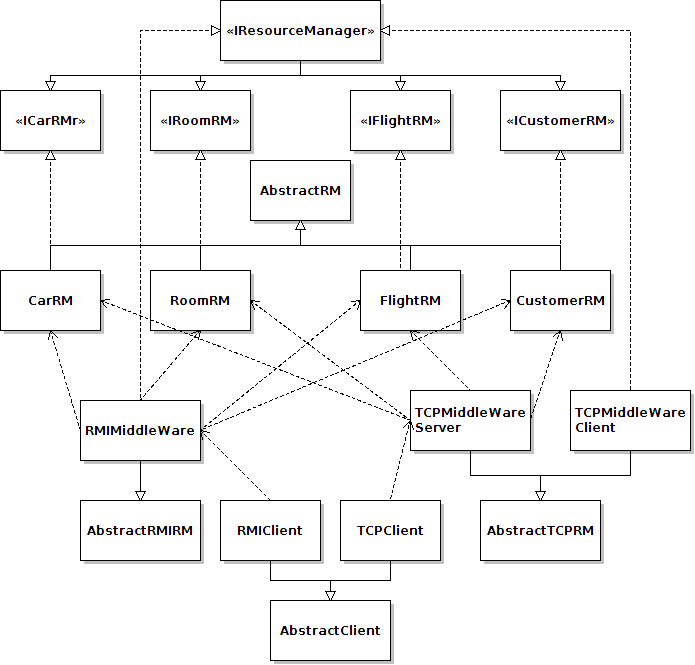
\includegraphics[scale=0.6,angle=90]{classhierarchy.png}
  \caption{UML Class Diagram}
  \label{uml}
\end{figure}


\subsection{Testing}
\subsubsection{Bash scripts}
To facilitate the testing of the system, Bash scripts are available.
\begin{itemize}
\item{
{\tt launch.sh [tcp/rmi] [car/room/flight/middleware] [port] [.....]}.

It take several arguments to launch each of the service (CarResourceManager,Room,Flight,Middleware or Client), either via TCP or RMI.
}
\item{
{\tt launch-localhost.sh [tcp/rmi] [portcar] [portroom] [portflight] [portmiddleware]}.

It deploys all the services all at a time on localhost.
}
\item{
{\tt launch-client.sh [tcp/rmi] [host:port]} is used to launch a client (either RMI or TCP) 
allowing fast testing when it's combined with the {\tt input1} file which contains multiple testcases.
}
\end{itemize}

\subsubsection{Example}
A traditional runcase with 3 servers would be :

First, login to server1 and launch all the resource managers.

{\tt ./launch.sh rmi flight 2000}

{\tt ./launch.sh rmi car 2001}

{\tt ./launch.sh rmi room 2002}

Then, login to server2 and launch the middleware.

{\tt ./launch.sh rmi middleware 2003 -flight=server1:2000 -car=server1:2001 -room=server1:2002}

Finaly, login to server3 and use the client redirecting stdin from the input1 file
 
{\tt ./launch-client.sh rmi server2:2003 < input1}



%\bibliographystyle{plain}
%\bibliography{bib}
\end{document}
